\chapter{Introduction}

\section{Contexte}

Dans le cadre de ma 4\up{ème} année d'étude à Polytech Grenoble en informatique, j'ai effectué mon stage de 12 semaines à Universiti Teknologi PETRONAS (UTP) à Seri Iskandar, en Malaisie. Ce stage s'est déroulé du \textbf{20 mai 2019} au \textbf{9 août 2013}.

À l'occasion de la mise en place d'un futur parternariat entre Polytech Grenoble et UTP, différents sujets de stage nous ont été transmis par le bureau des relations internationnales de Polytech. Au final, nous sommes parti à quatre : j'ai été accompagné de deux autres étudiants venant de la spécialité INFO (Informatique) et un étudiant de IESE (Informatique et Electronique des Systèmes Embarqués).


\begin{figure}[h]
  \centering
  \begin{subfigure}{.5\textwidth}
    \centering
    
\includegraphics[width=.8\linewidth]{content/imgs/utp.jpg}
    \caption{Bibliothèque de l'université}
  \end{subfigure}%
  \begin{subfigure}{.5\textwidth}
    \centering
    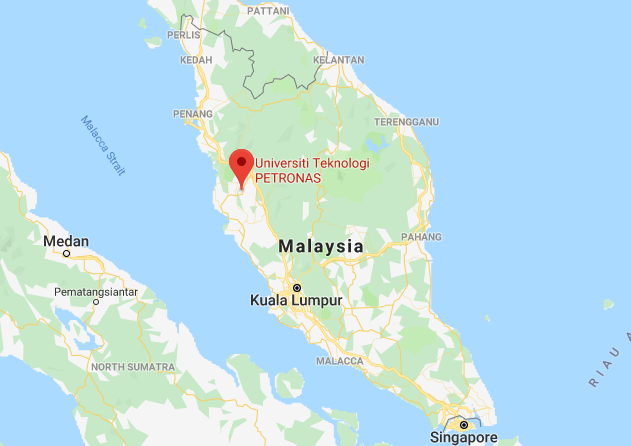
\includegraphics[width=.8\linewidth]{content/imgs/map.png}
    \caption{UTP, Seri Iskandar, Malaisie}
  \end{subfigure}
  \caption{Universiti Teknologi PETRONAS}
\end{figure}




\section{Sujet proposé}

Le sujet qui m'a été proposé a pour objectif de developper une application mobile dont le but est d'aider les personnes atteintent de bégaiement à guérir.

D'après \textit{Wikipédia}\cite{def_wiki}, le bégaiement est un trouble de la parole affectant le débit de la parole caractérisé par des répétitions et prolongations involontaires des sons, syllabes, mots ou phrases, et par des pauses silencieuses involontaires dans lequel le « bègue » (terme désignant un individu souffrant de bégaiement ou d'un trouble lié) est incapable de produire un son.

Une application similaire a déjà été développé durant trois années par des étudiants dans le cadre de leurs projet de fin d'étude. Comme illustré dans l'annexe \ref{appendix:old_app}, cette application propose les fonctionnalités suivantes :

\begin{itemize}
  \item Des exercices pour apprendre à contrôler son flux de parole ;
  \item La possibilité de visualiser sa progression pour chaque exercices (sour forme de liste, et pour certain exercices sous forme de graphique) ;
  \item Des informations concernant le bégaiement.
\end{itemize}

Cette application était disponible sur les appareils Android via le Play Store, la plateforme de téléchargement d'applications developpée par Google. Suite à un trop grand nombre de retours de \textit{bugs} concernant l'application, celle-ci a dû être retiré du Play Store.

Le sujet qui m'a été proposé est de recommencer depuis le début le developpement de cette application, en reprenant donc les fonctionnalités précédemment présentées.

Dans sa version finale, l'application devra donc proposer différents exercices pour apprendre à contrôler son flux de parole ainsi que la possibilité de visualiser sa progression pour chacun des exercices (avec des graphiques illustrant la progression de l'utilisateur). De plus, l'application pourra être utilisée par des orthophonistes pour accéder à la progression de leurs patients. Ils pourront laisser un commentaire sur les exercices effectuée par leurs partients pour les aider à progresser.

Aucune autre contrainte (technologie à utiliser, organisation de travail, etc.) m'a été imposée.


\section{But du rapport}
Ce rapport est destiné à tous ceux qui souhaite avoir un aperçu global du projet et de ce qui a été réalisé durant les 12 semaines consarcré à ce projet. En particulier, ce rapport est un bon point d'entrée pour tous ceux qui souhaite continuer le developpement de \textit{Stuttherapy}. Le rapport est disponible en anglais et en français.

\section{Organisation du rapport}

La rapport est tout d'abord constitué de cette partie, l'introduction. J'ai premièrement présenté le contexte dans lequelle le stage a été effectué puis dans un second temps j'ai donné une description succincte du sujet proposé.

Ensuite, la deuxième partie décrit le travail effectivement réalisé lors de ce stage, notamment tout le processus de réflexion, de recherches, de conception, d'organisation, de developpement et de tests.

Avant de conclure ce rapport, une page sera consacrée au developpement durable, en vertu de la loi Grenelle 1 de 2009 sur l'environnement.

Enfin, le bilan de ce rapport reviendra sur les connaissances que j'ai acquises et améliorées durant ces 12 semaines. J'y detaillerai les erreurs que j'ai commises, leurs causes et leurs conséquences.























%
